

\tikzset{every picture/.style={line width=0.75pt}} %set default line width to 0.75pt        

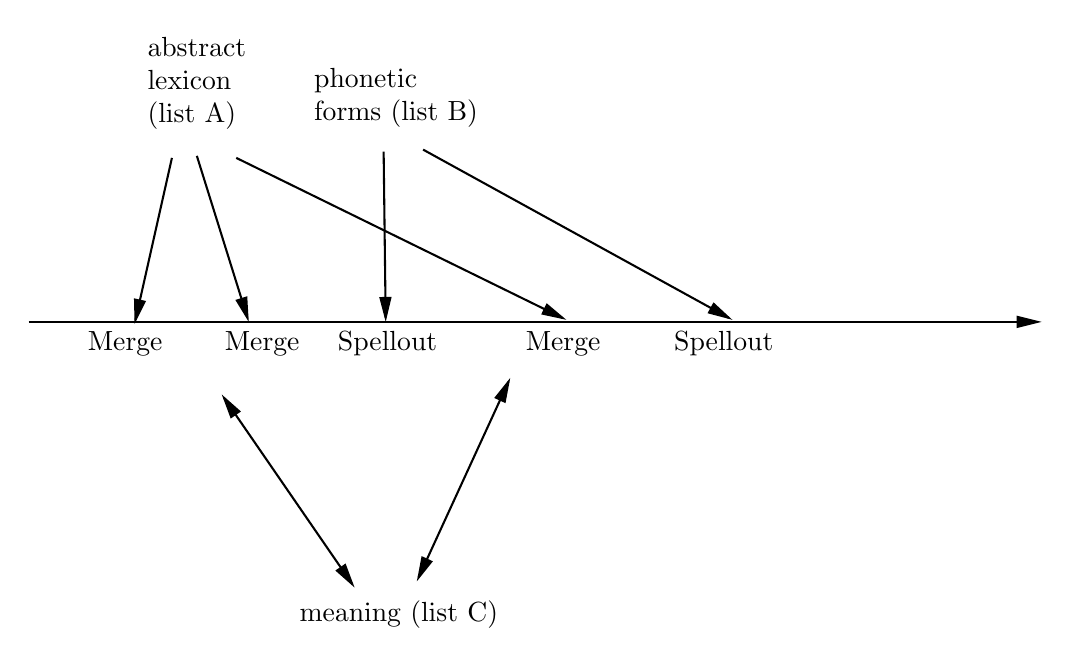
\begin{tikzpicture}[x=0.75pt,y=0.75pt,yscale=-1,xscale=1]
%uncomment if require: \path (0,335); %set diagram left start at 0, and has height of 335

%Straight Lines [id:da8133557183786788] 
\draw    (111,174) -- (597,174) ;
\draw [shift={(599,174)}, rotate = 180] [fill={rgb, 255:red, 0; green, 0; blue, 0 }  ][line width=0.08]  [draw opacity=0] (12,-3) -- (0,0) -- (12,3) -- cycle    ;
%Straight Lines [id:da9139623062429578] 
\draw    (180,95) -- (162.44,173.05) ;
\draw [shift={(162,175)}, rotate = 282.68] [fill={rgb, 255:red, 0; green, 0; blue, 0 }  ][line width=0.08]  [draw opacity=0] (12,-3) -- (0,0) -- (12,3) -- cycle    ;
%Straight Lines [id:da03470199826802922] 
\draw    (192,94) -- (216.4,172.09) ;
\draw [shift={(217,174)}, rotate = 252.65] [fill={rgb, 255:red, 0; green, 0; blue, 0 }  ][line width=0.08]  [draw opacity=0] (12,-3) -- (0,0) -- (12,3) -- cycle    ;
%Straight Lines [id:da44105963725312125] 
\draw    (282,92) -- (282.98,172) ;
\draw [shift={(283,174)}, rotate = 269.3] [fill={rgb, 255:red, 0; green, 0; blue, 0 }  ][line width=0.08]  [draw opacity=0] (12,-3) -- (0,0) -- (12,3) -- cycle    ;
%Straight Lines [id:da049869658230754954] 
\draw    (211,95) -- (368.2,172.12) ;
\draw [shift={(370,173)}, rotate = 206.13] [fill={rgb, 255:red, 0; green, 0; blue, 0 }  ][line width=0.08]  [draw opacity=0] (12,-3) -- (0,0) -- (12,3) -- cycle    ;
%Straight Lines [id:da31651729521748106] 
\draw    (301,91) -- (448.25,172.04) ;
\draw [shift={(450,173)}, rotate = 208.83] [fill={rgb, 255:red, 0; green, 0; blue, 0 }  ][line width=0.08]  [draw opacity=0] (12,-3) -- (0,0) -- (12,3) -- cycle    ;
%Straight Lines [id:da6422754162098989] 
\draw    (205.13,210.65) -- (266.87,300.35) ;
\draw [shift={(268,302)}, rotate = 235.47] [fill={rgb, 255:red, 0; green, 0; blue, 0 }  ][line width=0.08]  [draw opacity=0] (12,-3) -- (0,0) -- (12,3) -- cycle    ;
\draw [shift={(204,209)}, rotate = 55.47] [fill={rgb, 255:red, 0; green, 0; blue, 0 }  ][line width=0.08]  [draw opacity=0] (12,-3) -- (0,0) -- (12,3) -- cycle    ;
%Straight Lines [id:da8528940161688809] 
\draw    (342.17,202.82) -- (298.83,297.18) ;
\draw [shift={(298,299)}, rotate = 294.66] [fill={rgb, 255:red, 0; green, 0; blue, 0 }  ][line width=0.08]  [draw opacity=0] (12,-3) -- (0,0) -- (12,3) -- cycle    ;
\draw [shift={(343,201)}, rotate = 114.66] [fill={rgb, 255:red, 0; green, 0; blue, 0 }  ][line width=0.08]  [draw opacity=0] (12,-3) -- (0,0) -- (12,3) -- cycle    ;

% Text Node
\draw (192,59) node   [align=left] {abstract\\lexicon\\(list A)};
% Text Node
\draw (138,177) node [anchor=north west][inner sep=0.75pt]   [align=left] {Merge};
% Text Node
\draw (204,177) node [anchor=north west][inner sep=0.75pt]   [align=left] {Merge};
% Text Node
\draw (258.5,177) node [anchor=north west][inner sep=0.75pt]   [align=left] {Spellout};
% Text Node
\draw (288,66) node   [align=left] {phonetic\\forms (list B)};
% Text Node
\draw (349,177) node [anchor=north west][inner sep=0.75pt]   [align=left] {Merge};
% Text Node
\draw (420.5,177) node [anchor=north west][inner sep=0.75pt]   [align=left] {Spellout};
% Text Node
\draw (240,307) node [anchor=north west][inner sep=0.75pt]   [align=left] {meaning (list C)};


\end{tikzpicture}
